\section{Using Nemo as End User}

\subsection{User Authentication} 
When NEMO application is loaded, users are authenticated through username and password for login. Currently, there are two user roles (user and admin). Figure~\ref{fig:login-screen} shows NEMO sign in page.  

\begin{figure}[H]
\centering
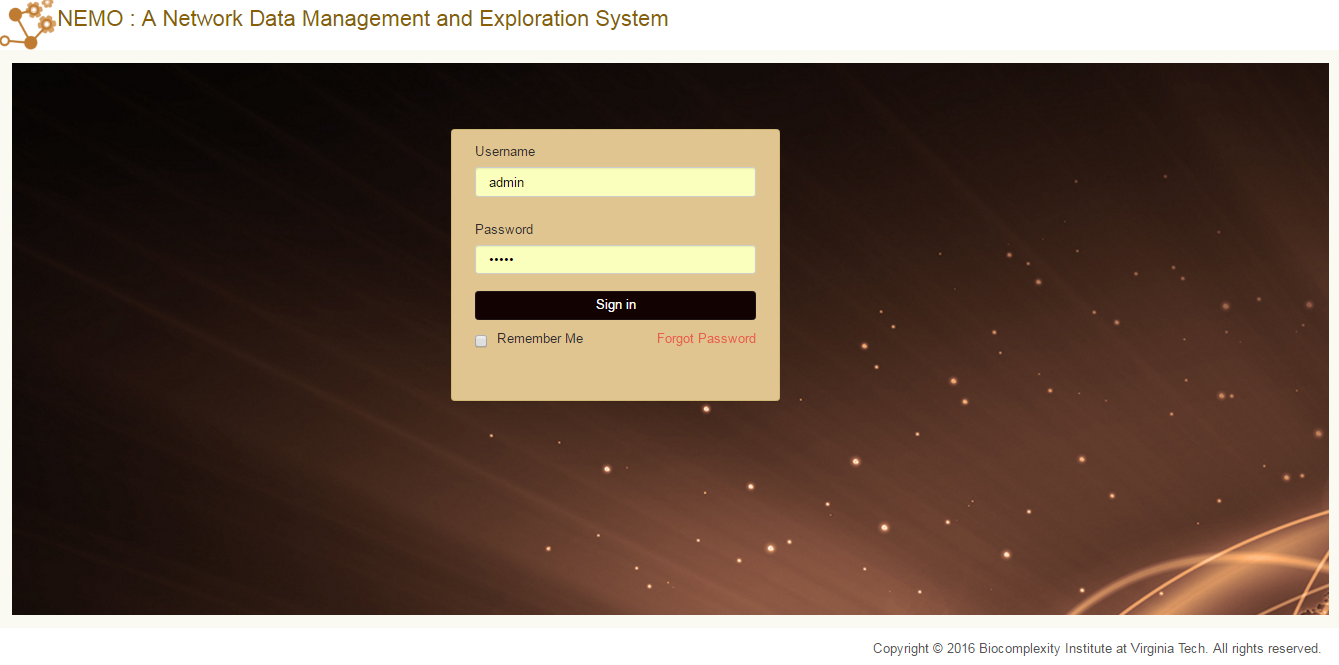
\includegraphics[trim = 0.0in 0.0in 0.0in 0.0in,scale=0.55]{login-screen}
\caption{
NEMO login page.
}   %   
\label{fig:login-screen}
\end{figure}

\subsection{Network Repository}
Once a user signed in, NEMO displays the network list view, see Figure~\ref{fig:network-list-screen}. There are two lists, a public list of networks added by current user and other users, where network is marked public. The other list contains networks owned by current user and might not necessarily be available for public. Users can search for a network by keyword(s) against a selected attribute (network name or description).

\begin{figure}[H]
\centering
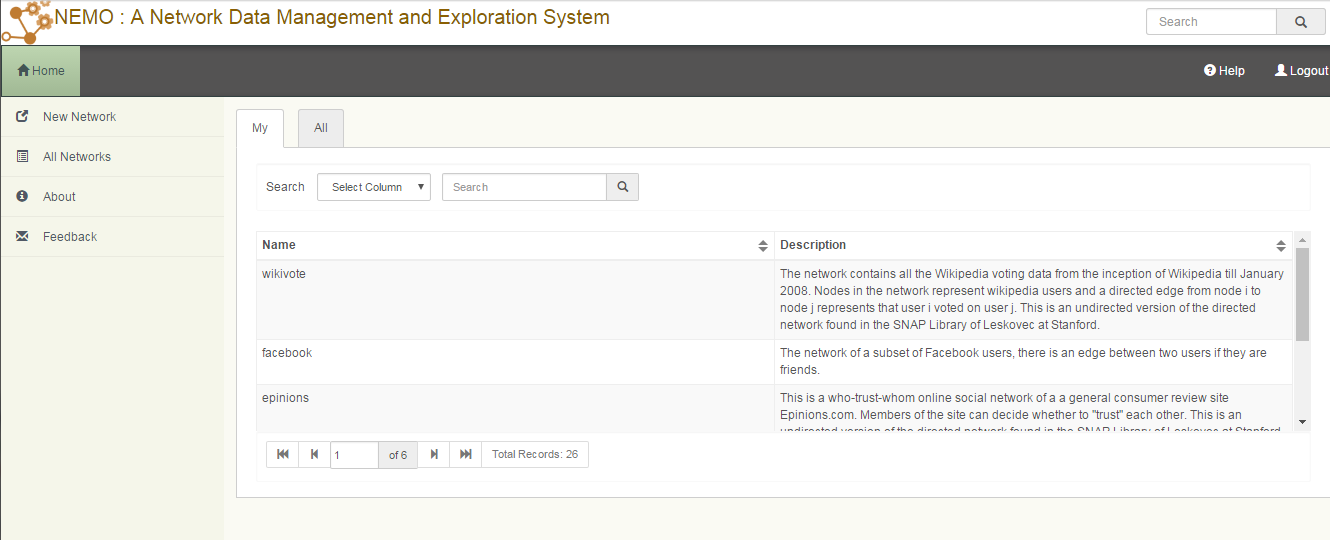
\includegraphics[trim = 0.0in 0.0in 0.0in 0.0in,scale=0.55]{network-list-screen}
\caption{
NEMO login page.
}   %   
\label{fig:network-list-screen}
\end{figure}


\subsection{Network Information}
By clicking on a network record in the network list, NEMO takes the user to another view that shows more detailed information including computer node and edge measures, see Figure. At any time users can proceed with further network visualization, analysis or return back to the network repository. 

\begin{figure}[H]
\centering
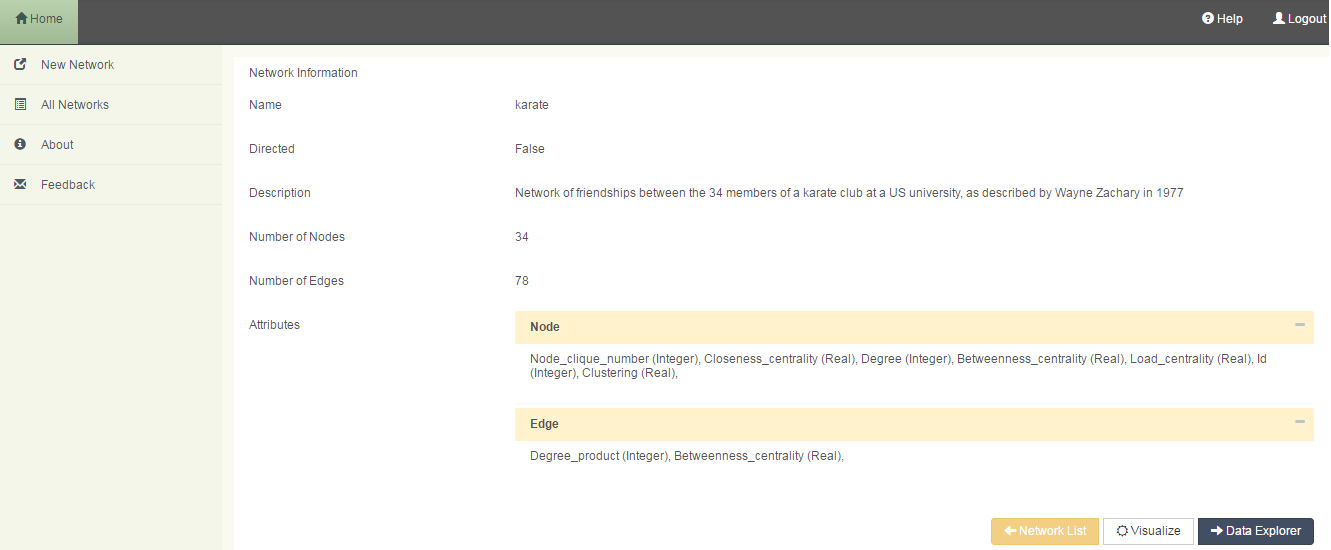
\includegraphics[trim = 0.0in 0.0in 0.0in 0.0in,scale=0.45]{network-info-screen2}
\caption{
Detailed information of a selected network Karate.
}   %   
\label{fig:network-info-screen2}
\end{figure}

\subsection{Network Visualization}
The visualization in Figure~\ref{fig:network-visualization3-screen} is generated with NEMO, using Gephi and a thin layer consisting of a Javascript GEXF
Viewer, available for download. Network visualization can be accessed through NEMO or directly through a supported separate URL. Visualizations can also be embedded into external websites. The visualization component resides on a separate machine from NEMO, which allows re-configuration or upgrading the visualization layer without affecting NEMO.
\begin{figure}[H]
\centering
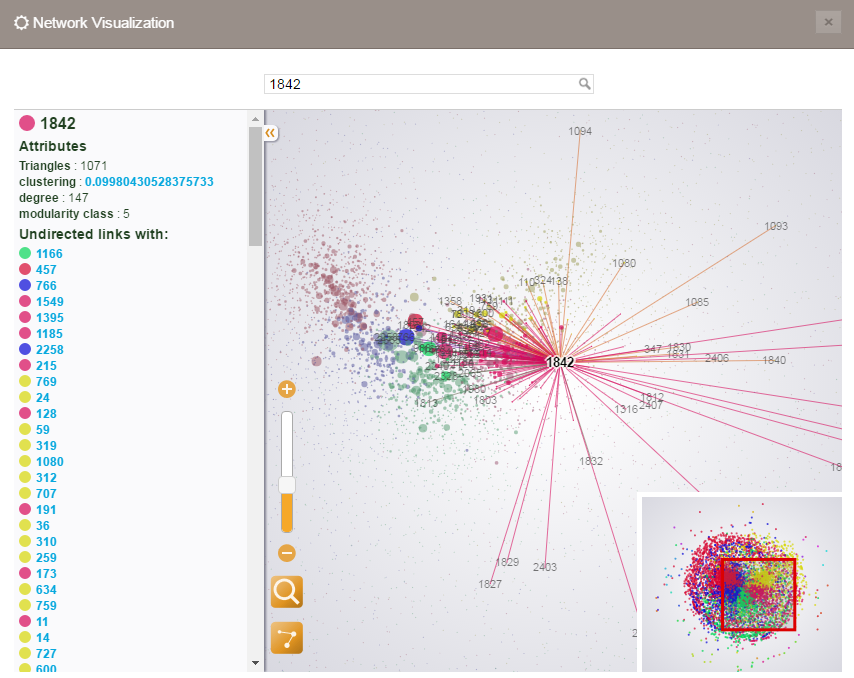
\includegraphics[trim = 0.0in 0.0in 0.0in 0.0in,scale=0.45]{network-visualization3-screen}
\caption{
Detailed information of a selected network Karate.
}   %   
\label{fig:network-visualization3-screen}
\end{figure}

\subsection{Data Explorer}

NEMO data explorer provides two ways for analyzing network data and reasoning about simulation results. The \textbf{query tab} allows the user to interact with MARS network query service. In addition to regular queries, user can run sampling queries for seed nodes/edges. Return data can be vertex IDs only, or IDs with all properties associated with
each vertex. Similarly for edge-based queries. This is useful for queries that produce large return sets; if all that is needed
are vertex (resp. edge) IDs, then much storage can be saved. Currently results can be copied to clipboard, but downloading the results is possible.

\begin{figure}[H]
\centering
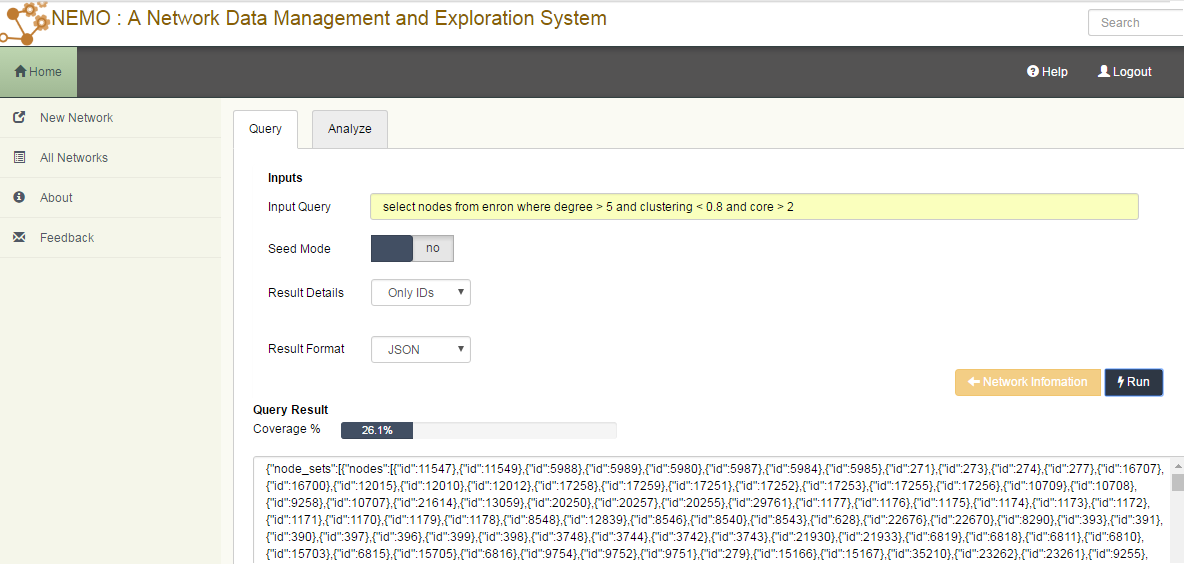
\includegraphics[trim = 0.0in 0.0in 0.0in 0.0in,scale=0.45]{network-query-screen-quality}
\caption{
NEMO screen for performing queries. The specified query returns all vertices that have degree > 5, clustering
coefficient < 0.8, and k-core of 3 or more. Result formats include JSON and XML. The particular
query returned 26.1% of network vertices.
}   %   
\label{fig:network-query-screen-quality}
\end{figure}

The \textbf{Analyze tab} provides a medium (workflow designer, see Figure~\ref{fig:network-wf-list-screen-new-5}) for users to construct workflows for network data analysis and plotting. 
\begin{figure}[H]
\centering
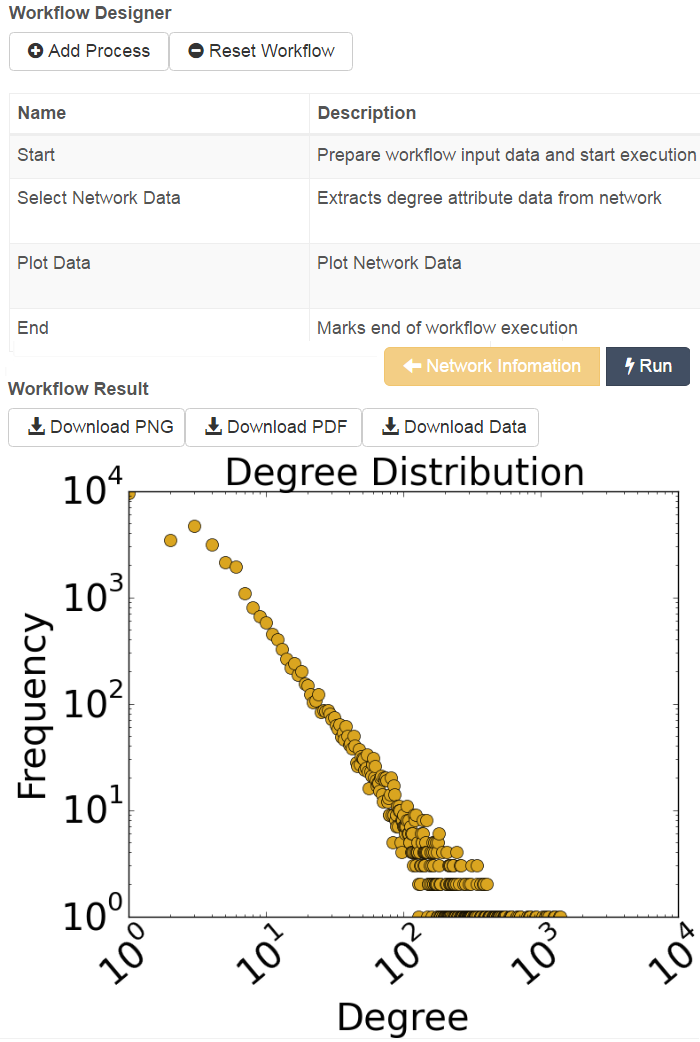
\includegraphics[trim = 0.0in 0.0in 0.0in 0.0in,scale=0.45]{network-wf-list-screen-new-5}
\caption{
NEMO workflow designer. User can add, edit or delete workflow processes in iterative manner. The final result can be numeric, text or plot. The generated plots are publication-quality and can be downloaded  in either pdf or png formats. Users can even download the plot raw data, if they want to use their own plotting tool.
}   %   
\label{fig:network-wf-list-screen-new-5}
\end{figure}
 
 \subsection{Examples of Plots can be generated by NEMO}
 
 \begin{figure}[H]
    \centering
    \begin{subfigure}[b]{0.3\textwidth}
        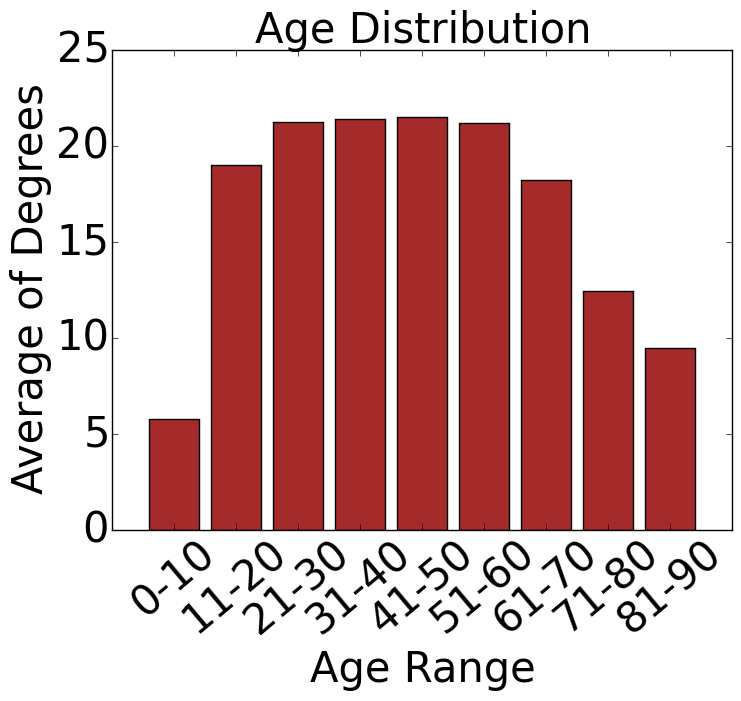
\includegraphics[width=\textwidth]{147}
        \caption{Average degree of a
person in each age bin.}
        \label{fig:147}
    \end{subfigure}
    ~ %add desired spacing between images, e. g. ~, \quad, \qquad, \hfill etc. 
      %(or a blank line to force the subfigure onto a new line)
    \begin{subfigure}[b]{0.3\textwidth}
        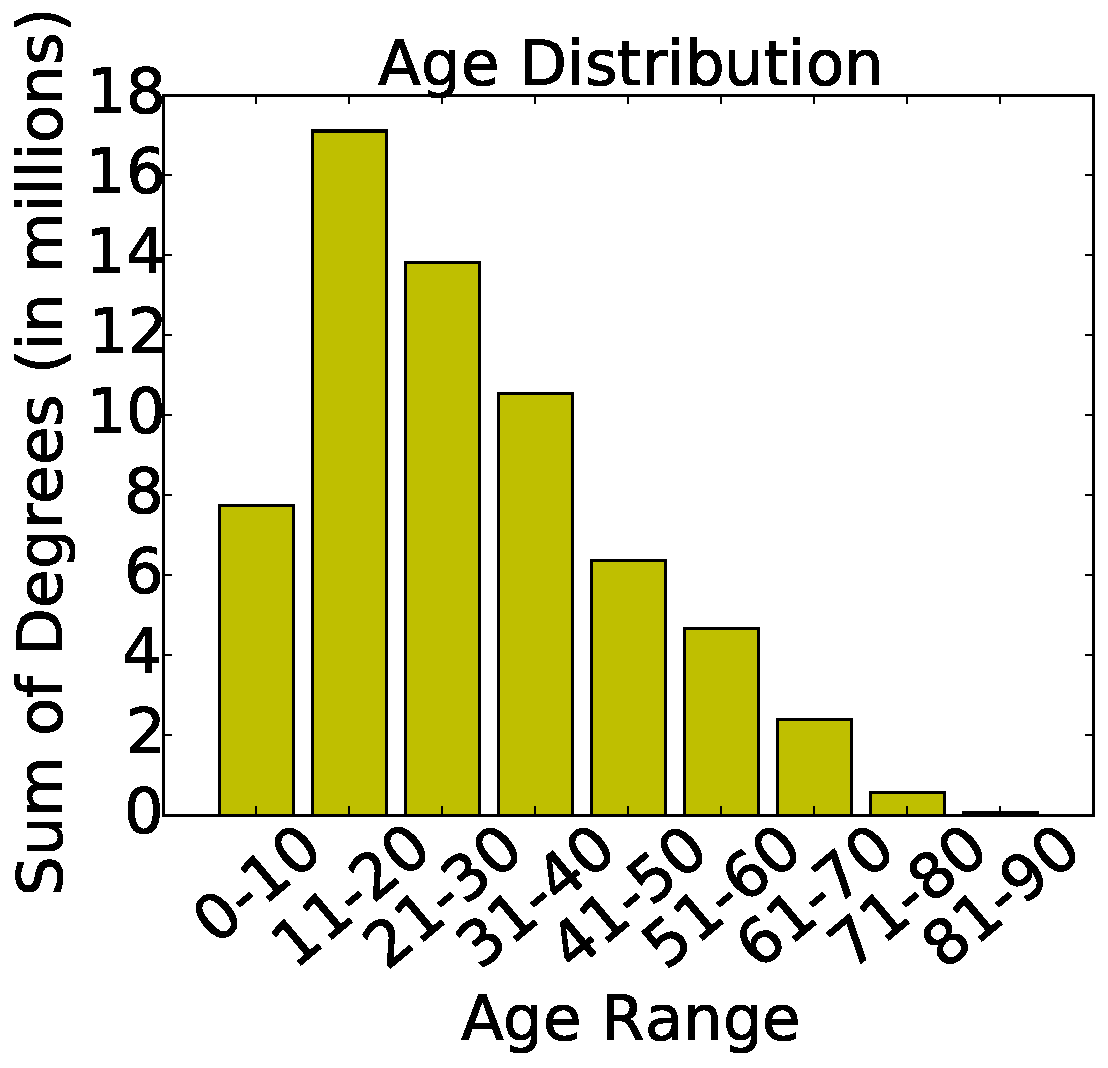
\includegraphics[width=\textwidth]{137}
        \caption{Total number of edges
formed by people in each age bin.}
        \label{fig:137}
    \end{subfigure}
    ~ %add desired spacing between images, e. g. ~, \quad, \qquad, \hfill etc. 
    %(or a blank line to force the subfigure onto a new line)
      \begin{subfigure}[b]{0.3\textwidth}
        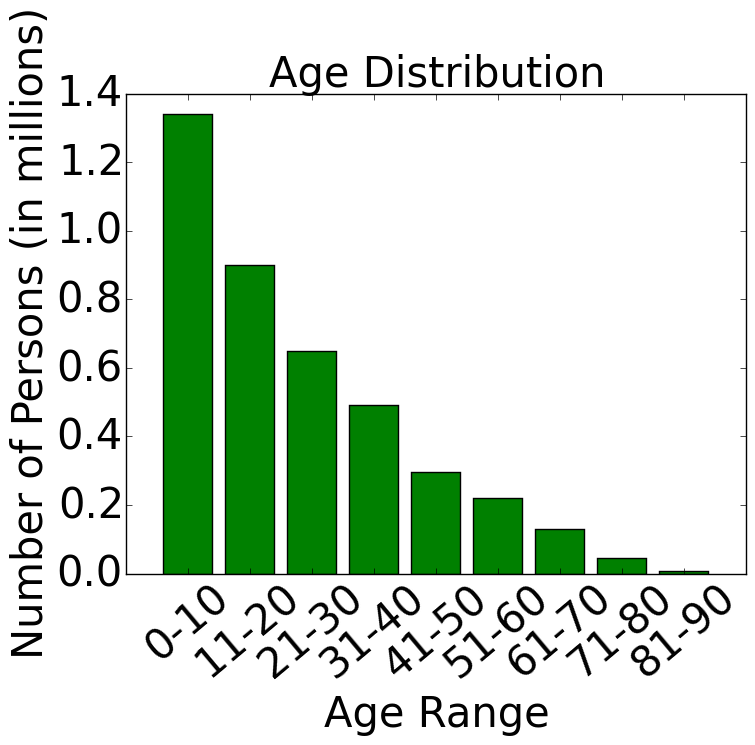
\includegraphics[width=\textwidth]{144}
        \caption{The number of people in each age range}
        \label{fig:144}
    \end{subfigure}
     \\
     \begin{subfigure}[b]{0.3\textwidth}
        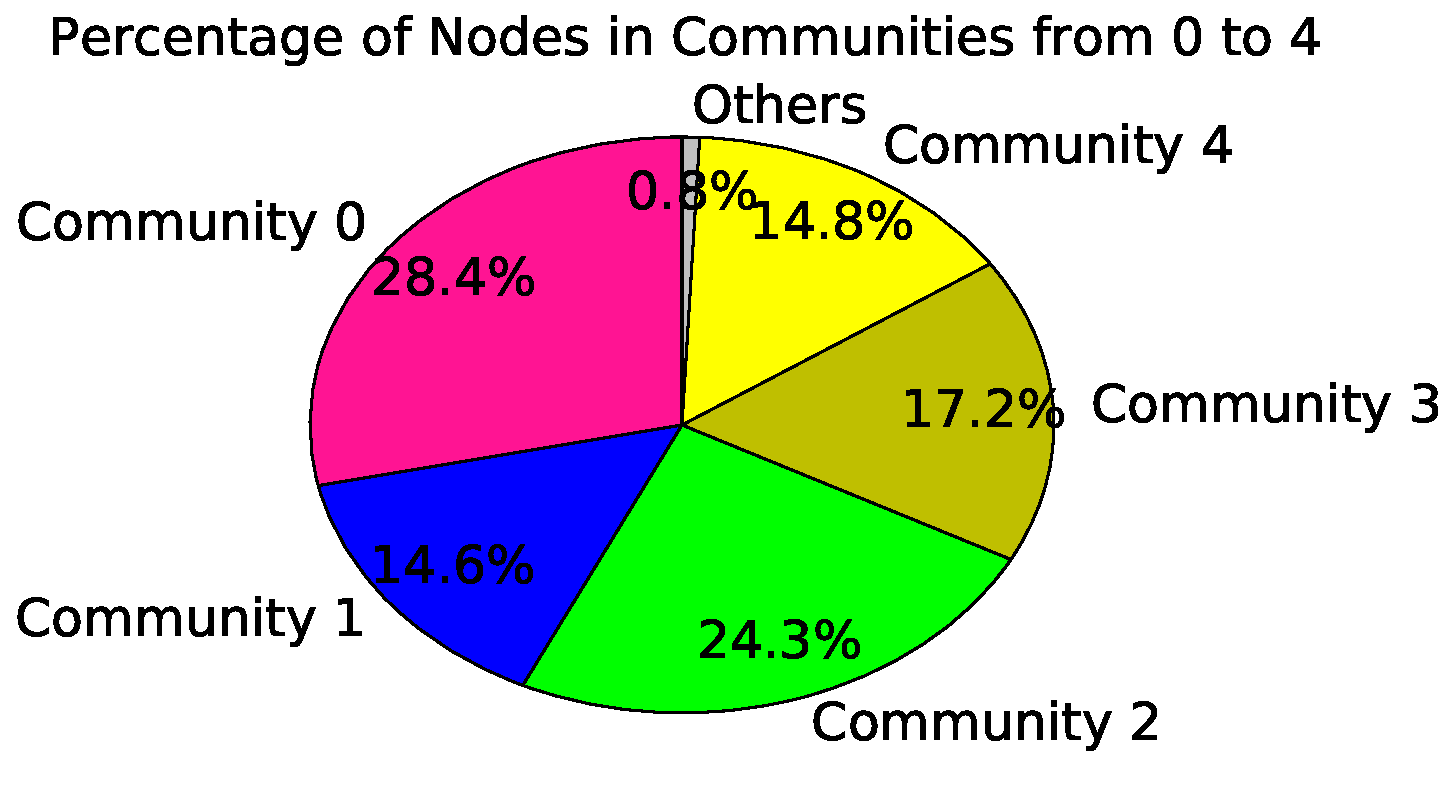
\includegraphics[width=\textwidth]{183}
        \caption{Fraction of vertices in each of the five largest communities
for a Wikivote network with 7115 vertices.}
        \label{fig:183}
    \end{subfigure}
    ~ 
     \begin{subfigure}[b]{0.3\textwidth}
        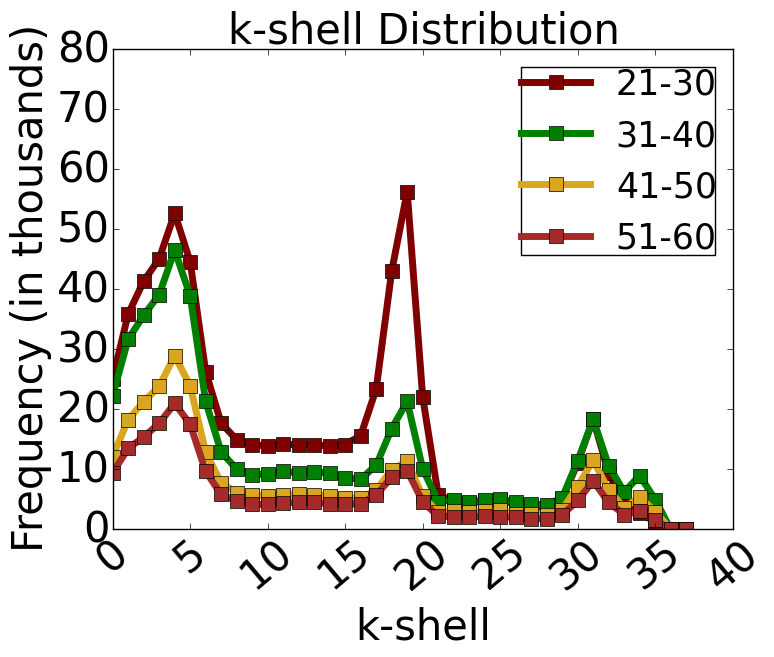
\includegraphics[width=\textwidth]{k-shell-1}
        \caption{The number of people in each age range, where the
ranges are 10-year increments.}
        \label{fig:k-shell-1}
    \end{subfigure}
    ~ 
     \begin{subfigure}[b]{0.3\textwidth}
        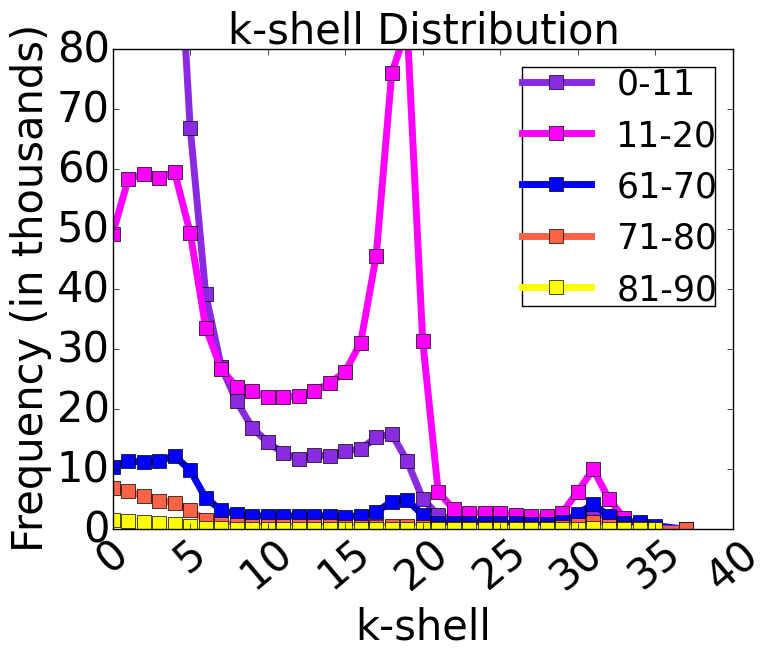
\includegraphics[width=\textwidth]{k-shell-2}
        \caption{The number of people in each age range, where the
ranges are 10-year increments.}
        \label{fig:k-shell-2}
    \end{subfigure}
    \\
    \begin{subfigure}[b]{0.3\textwidth}
        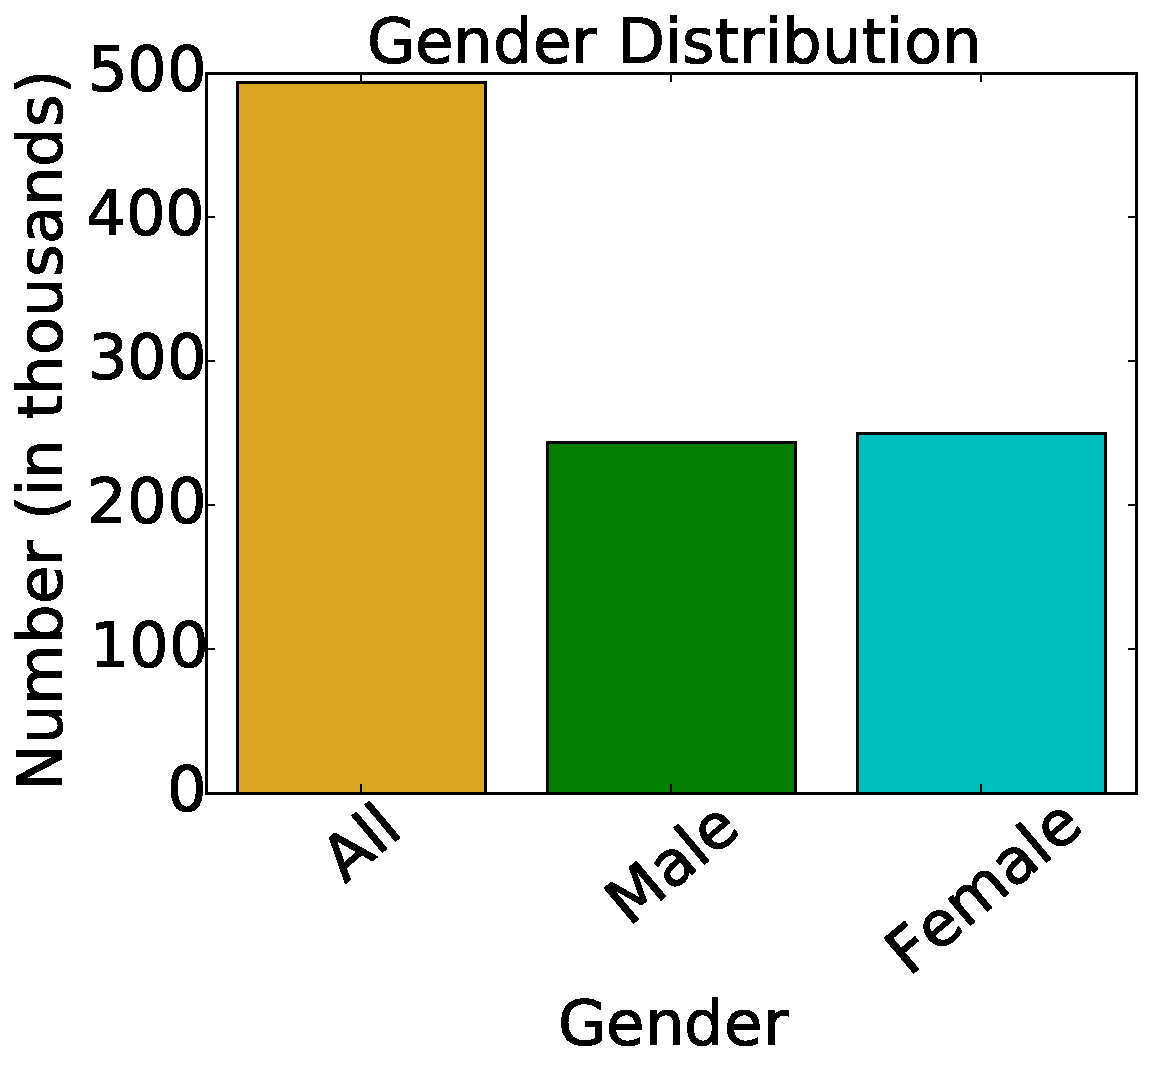
\includegraphics[width=\textwidth]{ebola-2}
        \caption{The number of people in each age range, where the
ranges are 10-year increments.}
        \label{fig:ebola-2}
    \end{subfigure}
    ~
    \begin{subfigure}[b]{0.3\textwidth}
        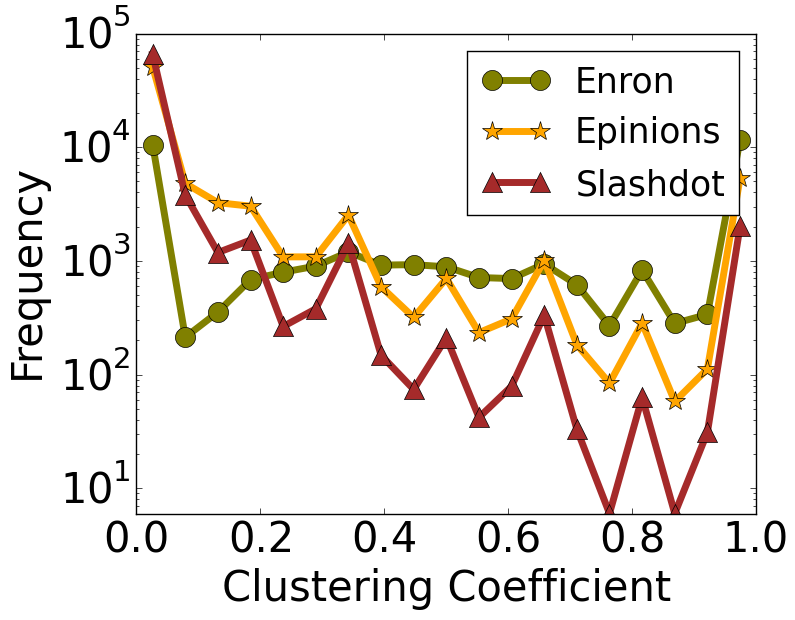
\includegraphics[width=\textwidth]{combined-clustering2}
        \caption{The number of people in each age range, where the
ranges are 10-year increments.}
        \label{fig:combined-clustering2}
    \end{subfigure}
    ~
    \begin{subfigure}[b]{0.3\textwidth}
        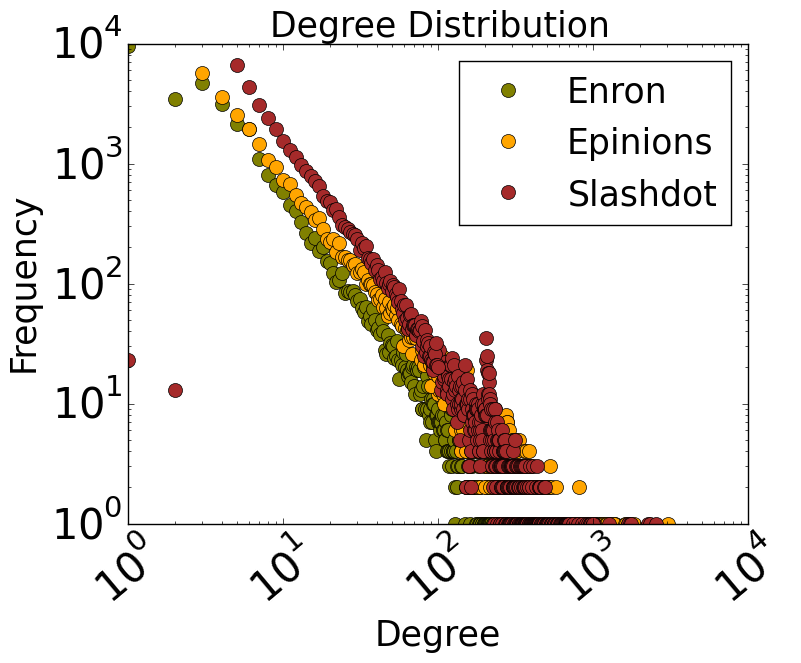
\includegraphics[width=\textwidth]{degree-combined}
        \caption{The number of people in each age range, where the
ranges are 10-year increments.}
        \label{fig:degree-combined}
    \end{subfigure}
    \caption{Different plots generated by NEMO workflows}\label{fig:nemo-plots}
\end{figure}